% Appendix draft for the thesis.
% Suggested usage: place this file after \appendix in the main thesis project,
% or copy selected chapters/sections into the existing appendix file.
% The figures are expected to be located under appendix_materials/figures/.

\chapter{Experimental Reproducibility Materials}

\section{Experimental Environment}

All experimental results reported in this thesis were obtained on a low-resource
Tencent Cloud CVM instance. The instance was configured with a 2-core CPU, 2 GB
of memory, and a 40 GB SSD cloud disk, running Ubuntu 24.04 LTS. The proposed
cardinality estimation framework was implemented in Java and built with Maven.
The experiments were executed under OpenJDK 17, and no GPU acceleration was used.
This environment was selected to approximate the limited computing and memory
resources available on edge-side nodes.

\section{Running Commands and Output Files}

The experimental program can be compiled and executed using the following
commands:

\begin{lstlisting}[language=bash]
mvn clean compile
mvn exec:java
\end{lstlisting}

After execution, the program exports two main result files:

\begin{itemize}
    \item \texttt{results\_summary.md}: aggregated results grouped by dataset,
    workload group, and estimation method;
    \item \texttt{results\_detail.csv}: per-query results, including the actual
    cardinality, estimated cardinality, relative error, Q-Error, inference time,
    throughput, and JVM heap memory increment.
\end{itemize}

In the appendix material folder, these two files are stored under
\texttt{data/}. The detailed CSV file is not printed in the thesis because it
contains 4800 experimental records, but it is retained as reproducibility
material.

\section{Dataset and Workload Parameters}

Table~\ref{tab:app_dataset_workload_parameters} summarizes the main dataset and
query workload parameters used in the experiments.

\begin{table}[htbp]
    \centering
    \caption{Dataset and workload generation parameters}
    \label{tab:app_dataset_workload_parameters}
    \small
    \begin{tabular}{ll}
        \toprule
        Parameter & Setting \\
        \midrule
        Datasets & \texttt{D2}, \texttt{D5} \\
        Records per dataset & 10000 \\
        Dimensionality & 2 and 5 \\
        Data distribution & Multi-cluster Gaussian distribution with white noise \\
        Number of Gaussian clusters & 5 \\
        Nominal attribute domain & $[1.0, 100.0]$ \\
        Query type & Multi-attribute conjunctive range query \\
        Workload groups & \texttt{narrow}, \texttt{medium}, \texttt{wide} \\
        Queries per group & 200 \\
        Queries per dataset & 600 \\
        Initial selectivity targets & $(0,0.05]$, $(0.10,0.30]$, $(0.50,1.00]$ \\
        Query half-width ratio & $[0.05, 0.40]$ of each attribute range \\
        Maximum attempts before relaxation & 50 \\
        Random seeds for workload groups & 1001, 1002, 1003 \\
        Ground truth cardinality & Exact full scan over the original dataset \\
        \bottomrule
    \end{tabular}
\end{table}

The workload group labels are nominal groups based on different initial
selectivity targets. Since the query generator may relax the target interval
when valid candidates are difficult to find, \texttt{narrow}, \texttt{medium},
and \texttt{wide} should not be interpreted as strict selectivity partitions.

\section{Implementation Modules}

Table~\ref{tab:app_project_modules} lists the main implementation modules used
to reproduce the experiments.

\begin{table}[htbp]
    \centering
    \caption{Main implementation modules}
    \label{tab:app_project_modules}
    \small
    \begin{tabular}{lll}
        \toprule
        Module & Main file & Function \\
        \midrule
        Data generation & \texttt{GaussianDataGenerator.java} & Generate synthetic datasets \\
        Query generation & \texttt{RangeQueryGenerator.java} & Generate range query workloads \\
        Proposed estimator & \texttt{ProposedEstimator.java} & Build and query the proposed estimator \\
        Baselines & \texttt{GlobalHistogramEstimator.java} & Build global histogram baselines \\
        Experiment runner & \texttt{ExperimentRunner.java} & Run experiments and export results \\
        Memory probe & \texttt{MemoryProbe.java} & Record approximate JVM heap increment \\
        \bottomrule
    \end{tabular}
\end{table}

\chapter{Supplementary Experimental Results}

\section{Supplementary Result Files}

The appendix material folder contains additional result tables and raw metrics
that support the analysis in Chapter 3:

\begin{itemize}
    \item \texttt{tables/cloud\_overall\_qerror\_table.tex}: LaTeX table for
    the overall Q-Error comparison;
    \item \texttt{tables/cloud\_efficiency\_table.tex}: LaTeX table for
    construction time, inference latency, throughput, and memory overhead;
    \item \texttt{tables/cloud\_overall\_and\_efficiency\_summary.csv}: compact
    machine-readable summary of accuracy and efficiency metrics;
    \item \texttt{tables/cloud\_group\_median\_metrics\_raw.csv}: grouped
    median Q-Error values for auxiliary workload observations.
\end{itemize}

The grouped results are provided only as supplementary observations. Because
the query generation procedure may relax the initial selectivity interval, the
grouped figures should not be used as strict selectivity-sensitivity evidence.

\section{Dataset Visualization}

Figure~\ref{fig:app_dataset_distribution} visualizes the two synthetic datasets.
The \texttt{D2} dataset is shown in its original two-dimensional space, while the
\texttt{D5} dataset is projected onto two dimensions using PCA for visualization.
The color indicates local point density.

\begin{figure}[htbp]
    \centering
    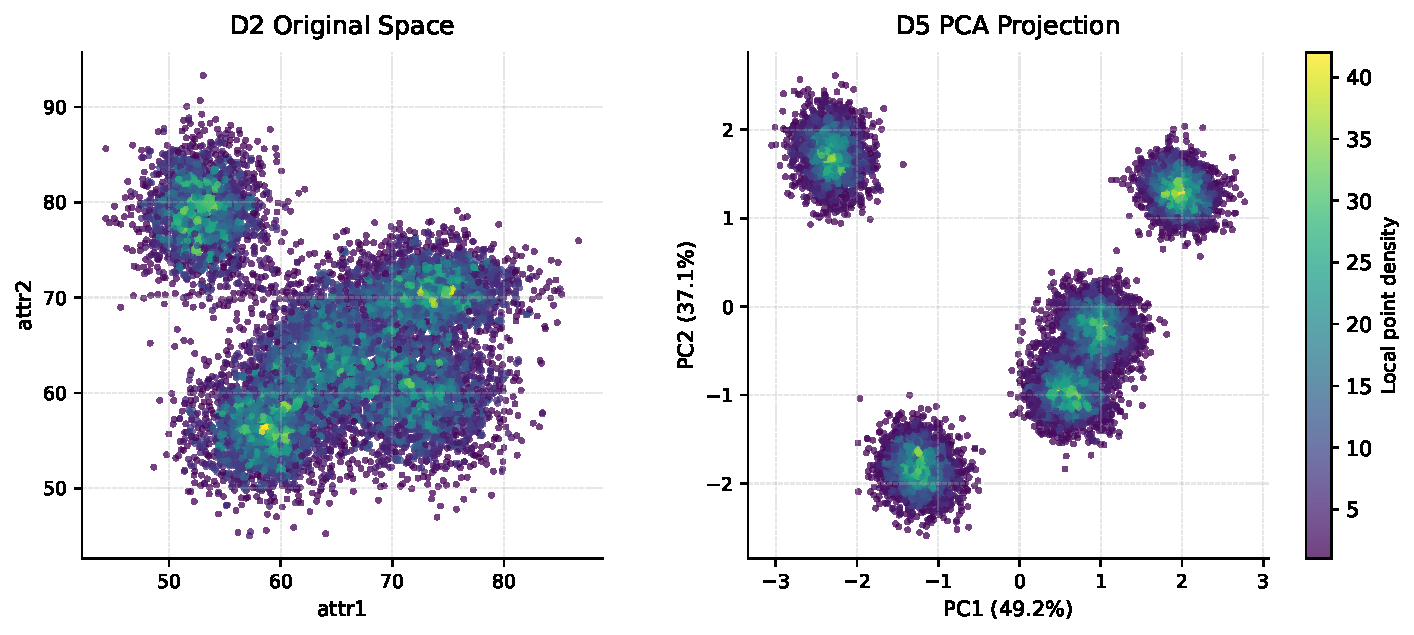
\includegraphics[width=0.92\textwidth]{figures/dataset_distribution_cloud}
    \caption{Visualization of synthetic datasets. \texttt{D2} is shown in its
    original space, while \texttt{D5} is shown using a two-dimensional PCA
    projection.}
    \label{fig:app_dataset_distribution}
\end{figure}

\section{Additional Accuracy Figures}

Figures~\ref{fig:app_overall_median_qerror}--\ref{fig:app_d5_qerror_boxplot}
provide supplementary visualizations of Q-Error results obtained on the Tencent
Cloud CVM instance.

\begin{figure}[htbp]
    \centering
    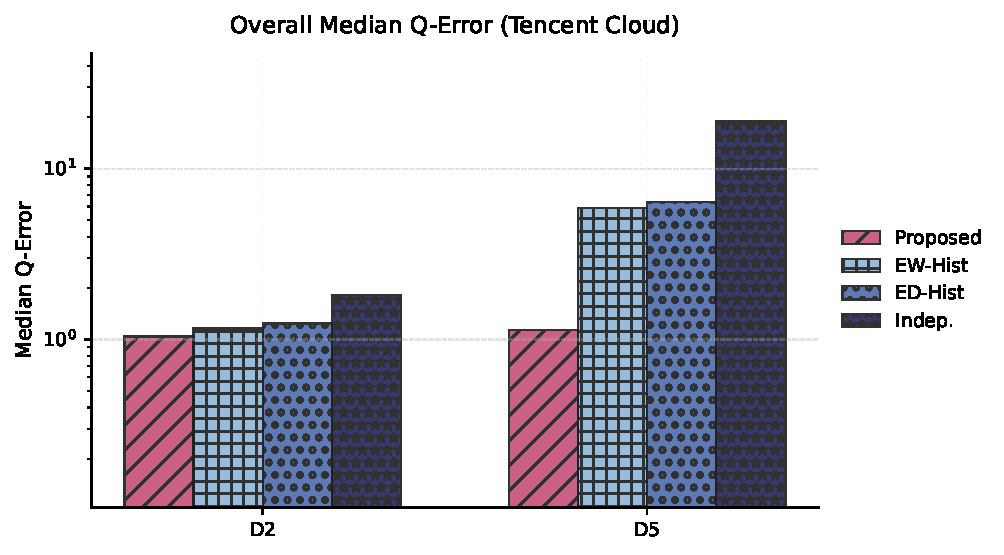
\includegraphics[width=0.78\textwidth]{figures/overall_median_qerror_cloud}
    \caption{Overall median Q-Error on \texttt{D2} and \texttt{D5}.}
    \label{fig:app_overall_median_qerror}
\end{figure}

\begin{figure}[htbp]
    \centering
    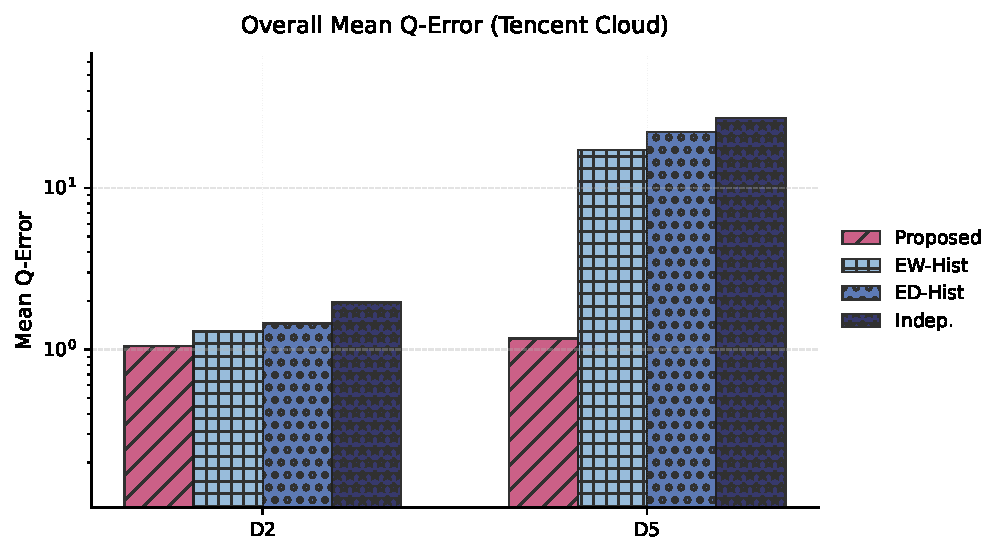
\includegraphics[width=0.78\textwidth]{figures/overall_mean_qerror_cloud}
    \caption{Overall mean Q-Error on \texttt{D2} and \texttt{D5}.}
    \label{fig:app_overall_mean_qerror}
\end{figure}

\begin{figure}[htbp]
    \centering
    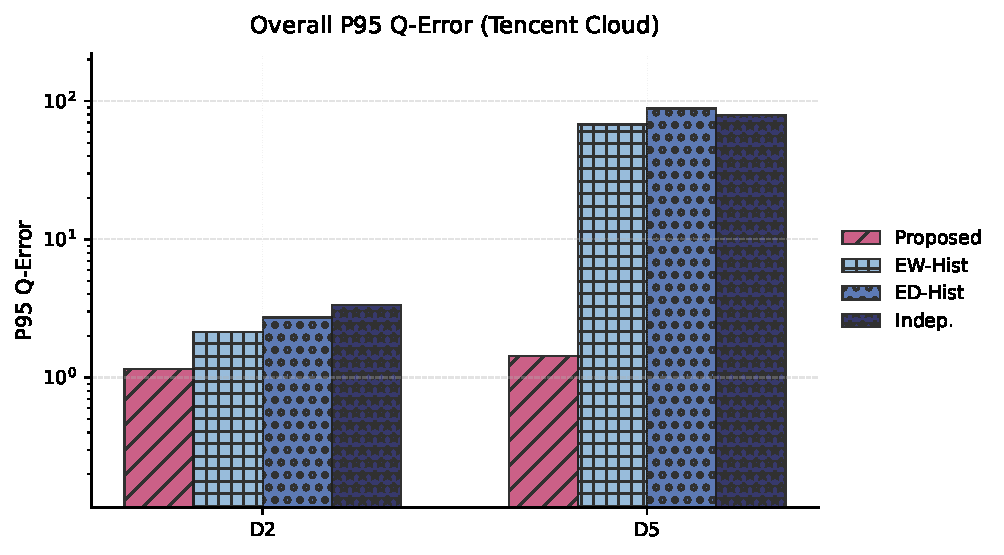
\includegraphics[width=0.78\textwidth]{figures/overall_p95_qerror_cloud}
    \caption{Overall P95 Q-Error on \texttt{D2} and \texttt{D5}.}
    \label{fig:app_overall_p95_qerror}
\end{figure}

\begin{figure}[htbp]
    \centering
    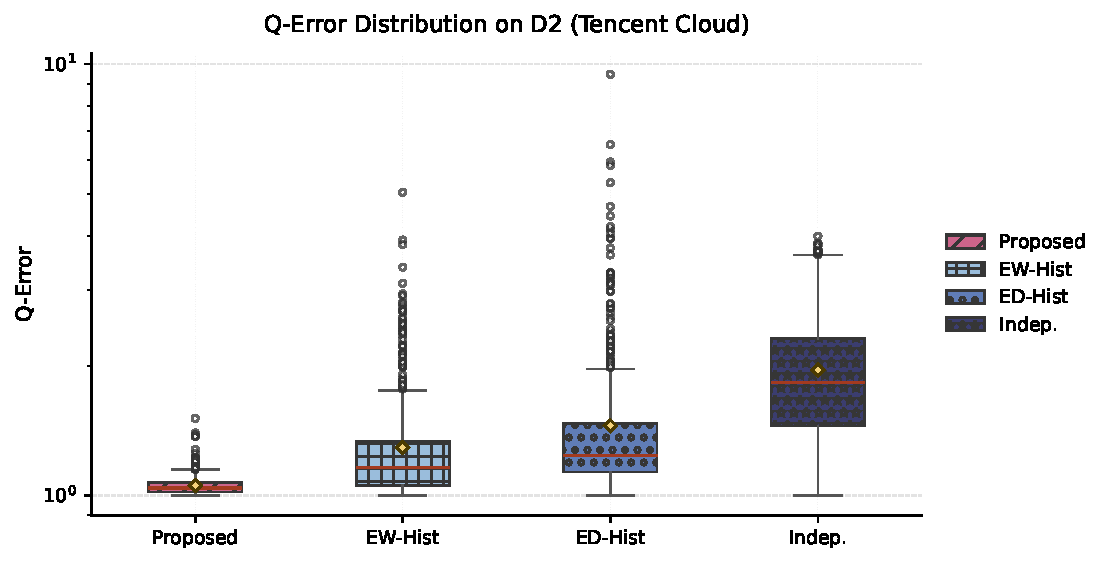
\includegraphics[width=0.82\textwidth]{figures/synthetic_D2_qerror_boxplot_qdspn_style_cloud}
    \caption{Q-Error distribution on \texttt{D2}.}
    \label{fig:app_d2_qerror_boxplot}
\end{figure}

\begin{figure}[htbp]
    \centering
    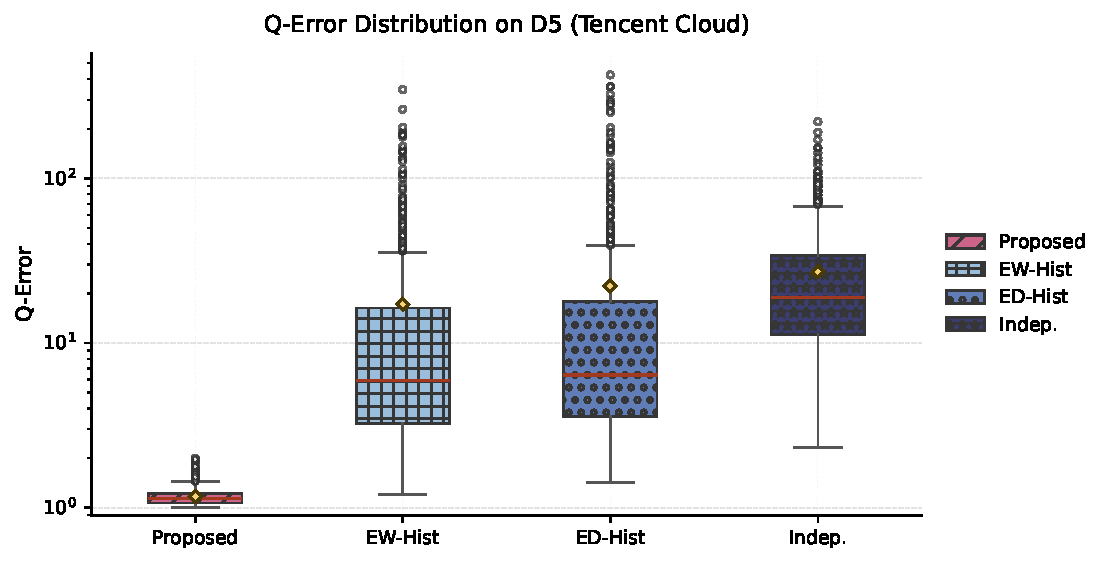
\includegraphics[width=0.82\textwidth]{figures/synthetic_D5_qerror_boxplot_qdspn_style_cloud}
    \caption{Q-Error distribution on \texttt{D5}.}
    \label{fig:app_d5_qerror_boxplot}
\end{figure}

\section{Additional Workload Group Figures}

Figures~\ref{fig:app_d2_group_median_qerror} and
\ref{fig:app_d5_group_median_qerror} show grouped median Q-Error values. These
figures are intended for auxiliary observation only, because the workload group
labels are nominal rather than strict selectivity partitions.

\begin{figure}[htbp]
    \centering
    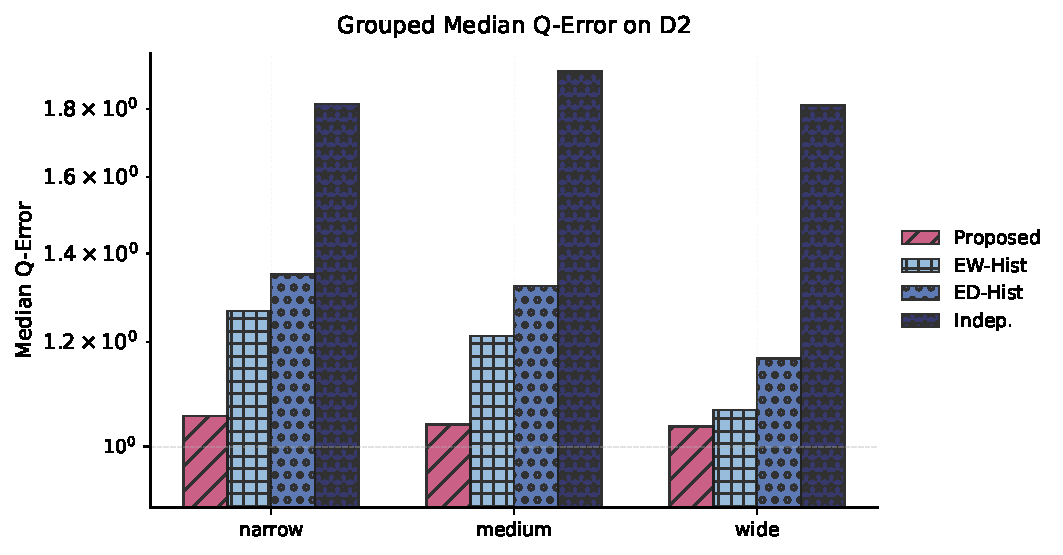
\includegraphics[width=0.78\textwidth]{figures/synthetic_D2_group_median_qerror_cloud}
    \caption{Grouped median Q-Error on \texttt{D2}.}
    \label{fig:app_d2_group_median_qerror}
\end{figure}

\begin{figure}[htbp]
    \centering
    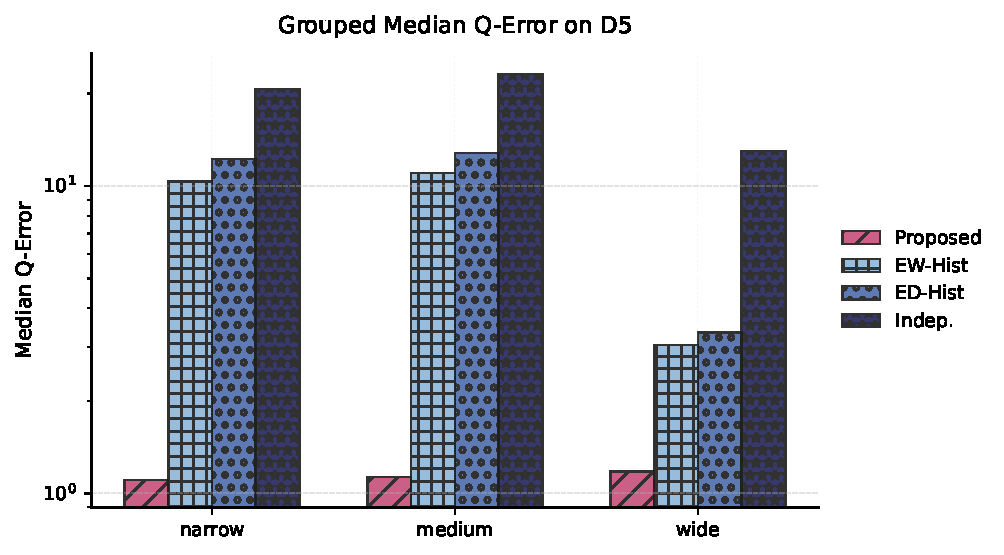
\includegraphics[width=0.78\textwidth]{figures/synthetic_D5_group_median_qerror_cloud}
    \caption{Grouped median Q-Error on \texttt{D5}.}
    \label{fig:app_d5_group_median_qerror}
\end{figure}

\section{Additional Efficiency Figures}

Figures~\ref{fig:app_fit_time}--\ref{fig:app_heap_overhead} provide
supplementary visualizations of construction time, inference latency, and JVM
heap memory increment.

\begin{figure}[htbp]
    \centering
    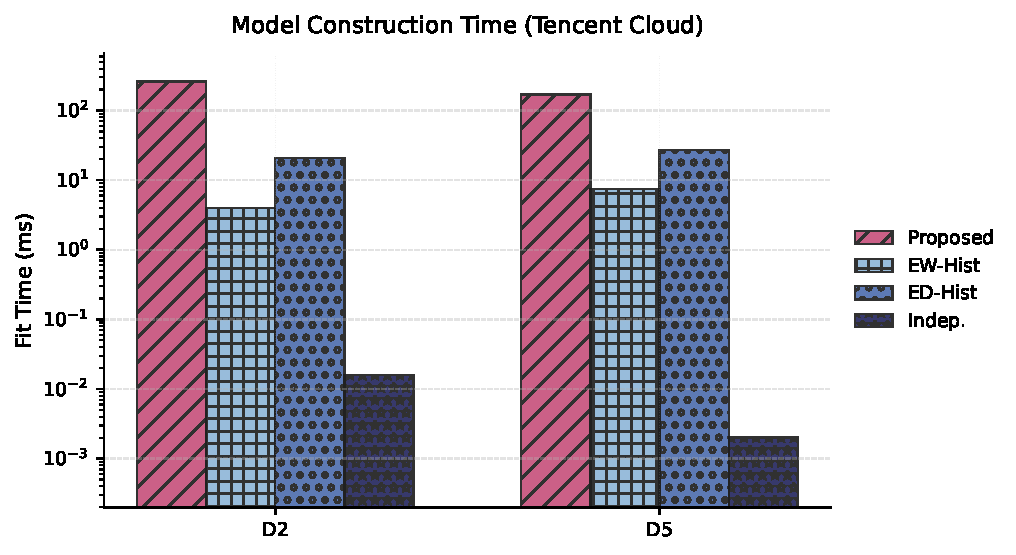
\includegraphics[width=0.78\textwidth]{figures/fit_time_cloud}
    \caption{Model construction time on \texttt{D2} and \texttt{D5}.}
    \label{fig:app_fit_time}
\end{figure}

\begin{figure}[htbp]
    \centering
    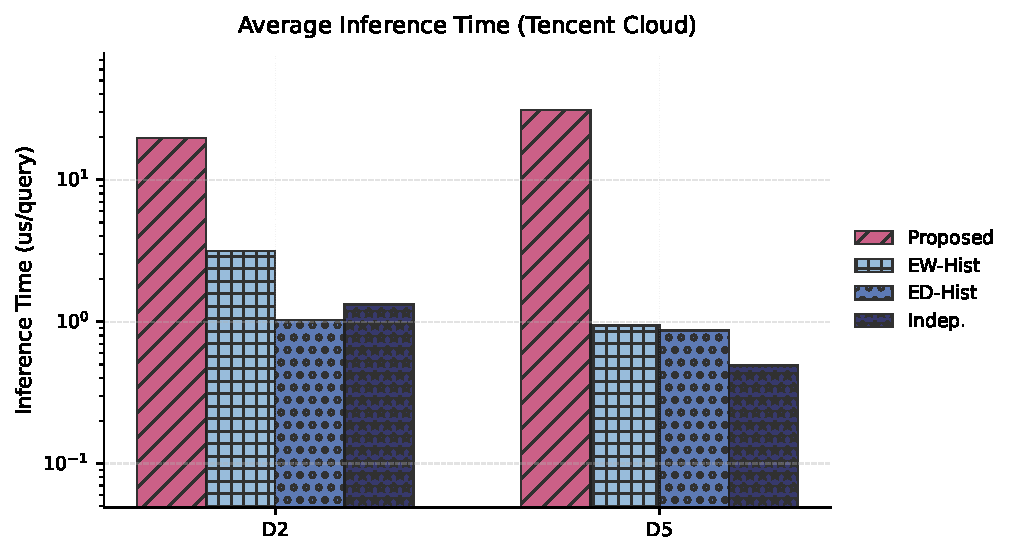
\includegraphics[width=0.78\textwidth]{figures/infer_time_cloud}
    \caption{Average inference time per query on \texttt{D2} and \texttt{D5}.}
    \label{fig:app_infer_time}
\end{figure}

\begin{figure}[htbp]
    \centering
    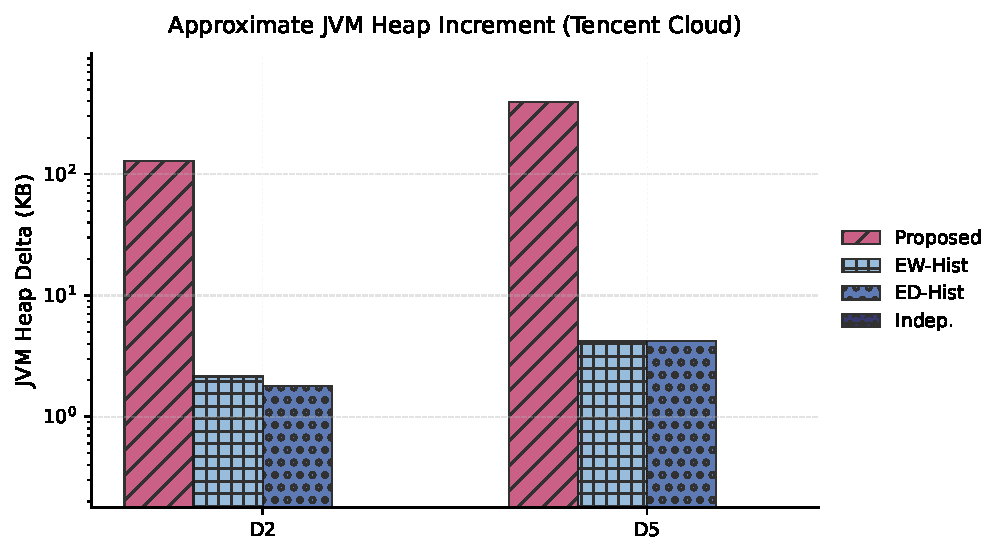
\includegraphics[width=0.78\textwidth]{figures/heap_overhead_cloud}
    \caption{Approximate JVM heap memory increment on \texttt{D2} and \texttt{D5}.}
    \label{fig:app_heap_overhead}
\end{figure}
